%%%%%%%%%%%%%%%%%%%%%%%%%%%%%%%%%%%%%%%%%%%%%%%%%%%%%%%%%%%%%%%%%%%%%%%%%%%%%%%%%%%%%%%%%%%%%%%%
%
% CS484 Written Question Template
%
% Acknowledgements:
% The original code is written by Prof. James Tompkin (james_tompkin@brown.edu).
% The second version is revised by Prof. Min H. Kim (minhkim@kaist.ac.kr).
%
% This is a LaTeX document. LaTeX is a markup language for producing 
% documents. Your task is to fill out this document, then to compile 
% it into a PDF document. 
%
% 
% TO COMPILE:
% > pdflatex thisfile.tex
%
% If you do not have LaTeX and need a LaTeX distribution:
% - Personal laptops (all common OS): www.latex-project.org/get/
% - We recommend latex compiler miktex (https://miktex.org/) for windows,
%   macTex (http://www.tug.org/mactex/) for macOS users.
%   And TeXstudio(http://www.texstudio.org/) for latex editor.
%   You should install both compiler and editor for editing latex.
%   The another option is Overleaf (https://www.overleaf.com/) which is 
%   an online latex editor.
%
% If you need help with LaTeX, please come to office hours. 
% Or, there is plenty of help online:
% https://en.wikibooks.org/wiki/LaTeX
%
% Good luck!
% Min and the CS484 staff
%
%%%%%%%%%%%%%%%%%%%%%%%%%%%%%%%%%%%%%%%%%%%%%%%%%%%%%%%%%%%%%%%%%%%%%%%%%%%%%%%%%%%%%%%%%%%%%%%%
%
% How to include two graphics on the same line:
% 
% \includegraphics[\width=0.49\linewidth]{yourgraphic1.png}
% \includegraphics[\width=0.49\linewidth]{yourgraphic2.png}
%
% How to include equations:
%
% \begin{equation}
% y = mx+c
% \end{equation}
% 
%%%%%%%%%%%%%%%%%%%%%%%%%%%%%%%%%%%%%%%%%%%%%%%%%%%%%%%%%%%%%%%%%%%%%%%%%%%%%%%%%%%%%%%%%%%%%%%%

\documentclass[11pt]{article}

\usepackage[english]{babel}
\usepackage[utf8]{inputenc}
\usepackage[colorlinks = true,
            linkcolor = blue,
            urlcolor  = blue]{hyperref}
\usepackage[a4paper,margin=1.5in]{geometry}
\usepackage{stackengine,graphicx}
\usepackage{fancyhdr}
\setlength{\headheight}{15pt}
\usepackage{microtype}
\usepackage{times}
\usepackage{booktabs}
\usepackage{listings}
\usepackage{xcolor}
\lstdefinestyle{codestyle}{
	frame=single,
	basicstyle=\ttfamily\footnotesize,
	keywordstyle=\bfseries\color{magenta},
	commentstyle=\itshape\color{gray},
	stringstyle=\color{orange},
	numberstyle=\sffamily\scriptsize\color{gray},
	showspaces=false,
	showstringspaces=false,
	showtabs=false,
	tabsize=4,
	breakatwhitespace=false,
	breaklines=true,
	keepspaces=true,
	captionpos=b,
	numbers=left,
	numbersep=5pt}
\lstset{style=codestyle}

\frenchspacing
\setlength{\parindent}{0cm} % Default is 15pt.
\setlength{\parskip}{0.3cm plus1mm minus1mm}

\pagestyle{fancy}
\fancyhf{}
\lhead{Homework Writeup}
\rhead{CS484}
\rfoot{\thepage}

\date{}

\title{\vspace{-1cm}Homework 3 Writeup}


\begin{document}
\maketitle
\vspace{-3cm}
\thispagestyle{fancy}

\section*{Instructions}
\begin{itemize}
  \item Describe any interesting decisions you made to write your algorithm.
  \item Show and discuss the results of your algorithm.
  \item Feel free to include code snippets, images, and equations.
  \item \textbf{Please make this document anonymous.}
\end{itemize}

\section*{Bayer Image Interpolation}

First part of this project is to make the code that interpolating the given bayer image into proper RGB image. 

\begin{lstlisting}[language=python]
def bayer_to_rgb_bilinear(bayer_img):
    
    height, width = bayer_img.shape
    rgb_img = np.zeros((height + 2, width + 2, 3), dtype=np.uint8)
    # added zero padding of 1 pixel width around the image for calculation efficiency    
    # Extract bayer image into each channel of rgb image
    # Range starts from 1 due to the padding
    rgb_img[1:-1:2, 1:-1:2, 0] = bayer_img[0::2, 0::2]    
    rgb_img[1:-1:2, 2:-1:2, 1] = bayer_img[0::2, 1::2]
    rgb_img[2:-1:2, 1:-1:2, 1] = bayer_img[1::2, 0::2]
    rgb_img[2:-1:2, 2:-1:2, 2] = bayer_img[1::2, 1::2]

    # For the R channel
    rgb_img[1:height:2, 2:width+1:2, 0] = (rgb_img[1:height:2, 1:width:2,0]//2 + 
    rgb_img[1:height:2, 3:width+2:2,0]//2) 
    rgb_img[2:height+1:2, 1:width:2, 0] = (rgb_img[1:height:2, 1:width:2,0]//2 + 
    rgb_img[3:height+2:2, 1:width:2,0]//2) 

    rgb_img[2:height+1:2, 2:width+1:2, 0] = (
        rgb_img[1:height:2, 1:width:2, 0]//4 + rgb_img[1:height:2, 3:width+2:2, 0]//4 +
        rgb_img[3:height+2:2, 1:width:2, 0]//4 + rgb_img[3:height+2:2, 3:width+2:2, 0]//4
    ) 
    #For the G channel
    rgb_img[1:-1:2, 1:-1:2, 1] = (
        rgb_img[1:-1:2, 0:-2:2, 1]//4 + 
        rgb_img[0:-2:2, 1:-1:2, 1]//4 +
        rgb_img[2::2, 1:-1:2, 1]//4 + 
        rgb_img[1:-1:2, 2::2, 1]//4
    )
    rgb_img[2:height+1:2, 2:width+1:2, 1] = (
        rgb_img[2:height+1:2, 1:width:2, 1]//4 + 
        rgb_img[1:height:2, 2:width+1:2, 1]//4 +
        rgb_img[3:height+2:2, 2:width+1:2, 1]//4 + 
        rgb_img[2:height+1:2, 3:width+2:2, 1]//4
    )

    # For the B channel
    rgb_img[2::2, 1:-2:2, 2] = (rgb_img[2::2, 0:-3:2,2]//2 +
    rgb_img[2::2, 2:-1:2,2]//2) 
    
    rgb_img[1:-2:2, 2::2, 2] = (rgb_img[0:-3:2, 2::2,2]//2 +
    rgb_img[2:-1:2, 2::2,2]//2) 
    
    rgb_img[1:-2:2, 1:-2:2, 2] = (
        rgb_img[0:-3:2, 0:-3:2, 2]//4 + 
        rgb_img[0:-3:2, 2:-1:2, 2]//4 +
        rgb_img[2:-1:2, 0:-3:2, 2]//4 + 
        rgb_img[2:-1:2, 2:-1:2, 2]//4
    )    
    #Remove Padding
    rgb_img = rgb_img[1:-1, 1:-1, :]
    
    return rgb_img
    \end{lstlisting}


\section*{Interesting Implementation Detail}

I'll explain my code step by step. 


\begin{enumerate}
    \item First, I made the empty array for result image with 2 pixels bigger than bayer image. This is because I wanted to add zero padding of 1 pixel around the image, for edge calculation.
    \item Then I brought the each R,G,B pixels from the bayer image and applied to channels in R,G,B order. To apply padding, i left the first and last pixels zero and filled the pixel value starting from 1.
    \item For each channel, used bilinear interpolation to fill the missing pixel values. I used indexing and slicing of Numpy to do this, since it is much faster than naive for loops.
    \item For the pixels in edges, I just used the same ways with other pixels, the only difference is that averaged the zero padding together. This makes the edge value smaller than intended, but it could the code more precise.
    \item Finally, I removed the zero padding by slicing the result image from the first pixel to the second last pixel.
\end{enumerate}

These are two images obatained from bilinear interpolation.

\begin{figure}
    \centering
    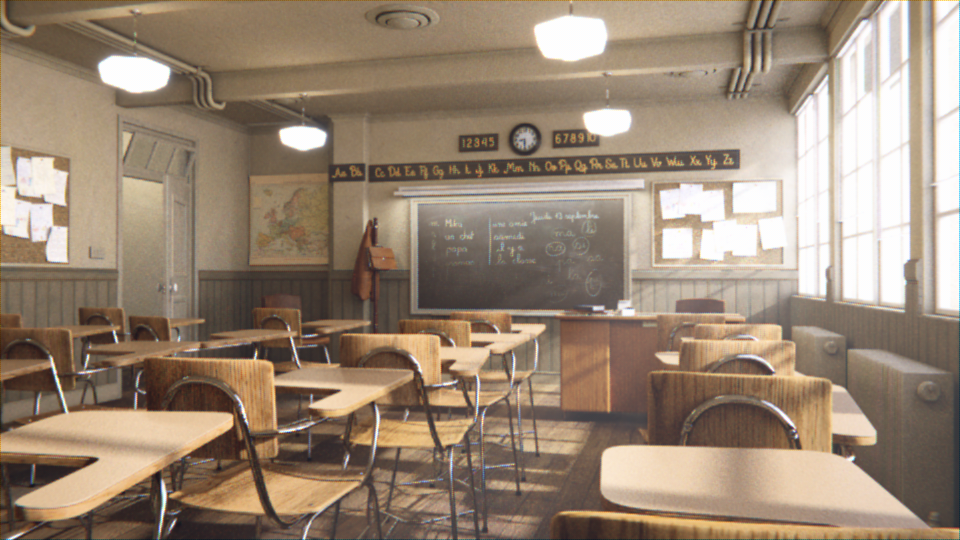
\includegraphics[width=5.5cm]{/Users/treblocami/Desktop/job/cs484_project/hw3_2023f/result/bilinear_img1.png}
    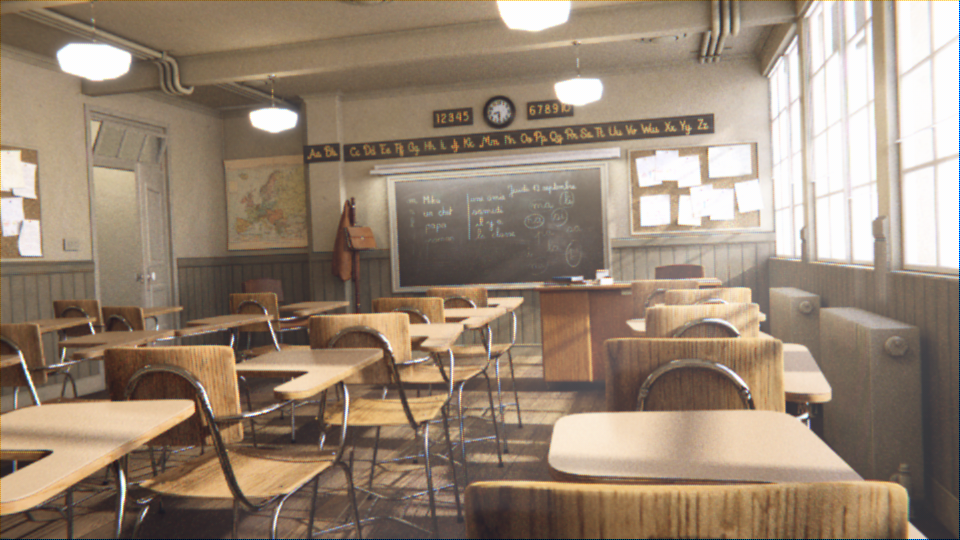
\includegraphics[width=5.5cm]{/Users/treblocami/Desktop/job/cs484_project/hw3_2023f/result/bilinear_img2.png}
\caption{Images obtained from bilienear interpolation}
\end{figure}

The problem in this implementation is as mentioned, the edge control. I think this could be resolved by using other methods for edges, such as reflection.


\section*{Fundamental Matrix Calculation}
In this section, with given 8 points on both images I obtained the fundamental matrix, using eight-point algorithm.

\begin{lstlisting}[language=python]
def calculate_fundamental_matrix(pts1, pts2):
    assert pts1.shape[1] == 2 and pts2.shape[1] == 2
    assert pts1.shape[0] == pts2.shape[0]
    
    n = pts1.shape[0]
    
    # Normalization
    mean1 = np.mean(pts1, axis=0)
    mean2 = np.mean(pts2, axis=0)
    
    scale1 = np.sqrt(2) / np.std(pts1)
    scale2 = np.sqrt(2) / np.std(pts2)
    
    T1 = np.array([
        [scale1, 0, -scale1 * mean1[0]],
        [0, scale1, -scale1 * mean1[1]],
        [0, 0, 1]
    ])
    
    T2 = np.array([
        [scale2, 0, -scale2 * mean2[0]],
        [0, scale2, -scale2 * mean2[1]],
        [0, 0, 1]
    ])
    
    pts1 = np.column_stack([pts1, np.ones(n)])
    pts2 = np.column_stack([pts2, np.ones(n)])

    pts1_normalized = (T1 @ pts1.T).T
    pts2_normalized = (T2 @ pts2.T).T
    
    A = np.zeros((n, 9))
    for i in range(n):
        x1, y1, _ = pts1_normalized[i]
        x2, y2, _ = pts2_normalized[i]
        A[i] = [x1*x2, x2*y1, x2, y2*x1, y1*y2, y2, x1, y1, 1]
    
    U, S, Vt = np.linalg.svd(A)
    f = Vt[-1]
    F = f.reshape(3, 3)
    
    U, S, Vt = np.linalg.svd(F)
    S[-1] = 0
    F = U @ np.diag(S) @ Vt
    
    # Denormalize
    F = T2.T @ F @ T1
    
    return F

def transform_fundamental_matrix(F, h1, h2):
    
    F_mod = np.linalg.inv(h2).T @ F @ np.linalg.inv(h1)
    
    return F_mod
\end{lstlisting}
\begin{enumerate}
    \item \textbf{Normalization:}
    First I normalized the given points using the built-in fuction $normalize\_points()$. 
    
    \item \textbf{Constructing Matrix A:}
    A matrix $A$ is constructed using the normalized points. Each row of $A$ is constructed as $[x_1'x_2, x_1'y_2, x_1', y_1'x_2, y_1'y_2, y_1', x_2, y_2, 1]$.
    
    \item \textbf{Singular Value Decomposition:}
    SVD is performed on matrix $A$ to find the Fundamental Matrix $F$.
    
    \item \textbf{Constraining $F$:}
    As $F$ is only determined up to a scale, and should have rank 2, the smallest singular value is set to zero to enforce this property.
    
    \item \textbf{Denormalization:}
    Finally, the Fundamental Matrix $F$ is denormalized to bring it back to the scale of the original points.
\end{enumerate}

\begin{enumerate}
    \item Result 1 was a total failure, because...
    \item Result 2 (Figure~\ref{fig:result1}, left) was surprising, because...
    \item Result 3 (Figure~\ref{fig:result1}, right) blew my socks off, because...
\end{enumerate}

\begin{figure}[h]
    \centering
    
\includegraphics[width=5cm]{placeholder.jpg}
    
\includegraphics[width=5cm]{placeholder.jpg}
    \caption{\emph{Left:} My result was spectacular. \emph{Right:} Curious.}
    \label{fig:result1}
\end{figure}

My results are summarized in Table~\ref{tab:table1}.

\begin{table}[h]
    \centering
    \begin{tabular}{lr}
        \toprule
        Condition & Time (seconds) \\
        \midrule
        Test 1 & 1 \\
        Test 2 & 1000 \\
        \bottomrule
    \end{tabular}
    \caption{Stunning revelation about the efficiency of my code.}
    \label{tab:table1}
\end{table}

\end{document}